\chapter{Contexto}
\label{chap:contexto}

\lettrine{N}{este} apartado introdúcense o contexto relevante a este traballo que provee os conceptos básicos necesarios para a súa comprensión.
Para elo descríbese o campo da oftalmoloxía e a imaxe médica, así como o estado da arte en aliñamento de imaxes.
\section{Oftalmoloxía}
\label{sec:Oftalmoloxía}
A oftalmoloxía é a especialidade médica encargada do estudo e tratamento das enfermidades dos ollos, incluíndo o globo ocular, a súa musculatura, o sistema lagrimal e as pálpebras.
O ollo humano é un dos órganos dos que mais dependemos e maior cantidade de información sensorial aporta, así como un dos mais complexos do noso corpo \cite{kanski2011clinical}.

A importancia da oftalmoloxía radica non só no tratamento das enfermidades oculares, senón tamén na súa capacidade para proporcionar información valiosa sobre o estado de saúde xeral do paciente. 
A observación directa dos vasos sanguíneos e do tecido neuronal 'in vivo' permite aos oftalmólogos detectar signos precoces de diversas enfermidades sistémicas.
 Por exemplo, o glaucoma, que non presenta síntomas nas súas etapas iniciais, pode ser diagnosticado mediante exames regulares da presión ocular e do nervio óptico \cite{importglaucoma}.
 Esta capacidade de diagnóstico precoz fai da oftalmoloxía unha especialidade fundamental na prevención e no mantemento da saúde visual e xeral do paciente.

 \subsection{Anatomía do ollo humano}
\label{subsec:Anatomía do ollo humano}
O ollo encargase de captar a luz e transformala en impulsos eléctricos que se envían ao cerebro.
 Esta información é interpretada polo cerebro, que mediante mecanismos como a atención e a memoria, permite a percepción visual. \cite{eyefunct}
 O ollo humano está composto por varias estruturas, cada unha cunha función específica que permite a percepción visual. Entre elas destacan:

 \begin{itemize}
 \item Córnea e Cristalino: actúan xuntas para enfocar a luz na retina. A córnea, situada na parte exterior do ollo, proporciona maior parte da capacidade refractiva, mentres que o cristalino, unha lente flexible, axusta o enfoque para obxectos a diferentes distancias.
 \item Pupila e Iris: regulan a cantidade de luz que entra no ollo. O iris, a parte coloreada do ollo, expándese ou contráese para controlar o tamaño da pupila, o orificio central.
 \item Retina: unha capa de células sensibles á luz (fotorreceptores) que converten os estímulos luminosos en sinais eléctricas, procesados inicialmente na retina mesma.
 \item Nervio óptico: transporta as sinais eléctricas xeradas na retina ata o cerebro, onde se interpretan como imaxes.
 \item Disco óptico: tamén coñecido como "punto cego", é a área onde o nervio óptico sae do ollo; carece de fotorreceptores.
 \item Vasos sanguíneos: distribúen os nutrientes e o osíxeno necesarios á retina e eliminan os seus residuos metabólicos.
 \end{itemize}
\cite{visionyojo}, \cite{eyeanat}

\begin{figure}[ht!]
    \centering
    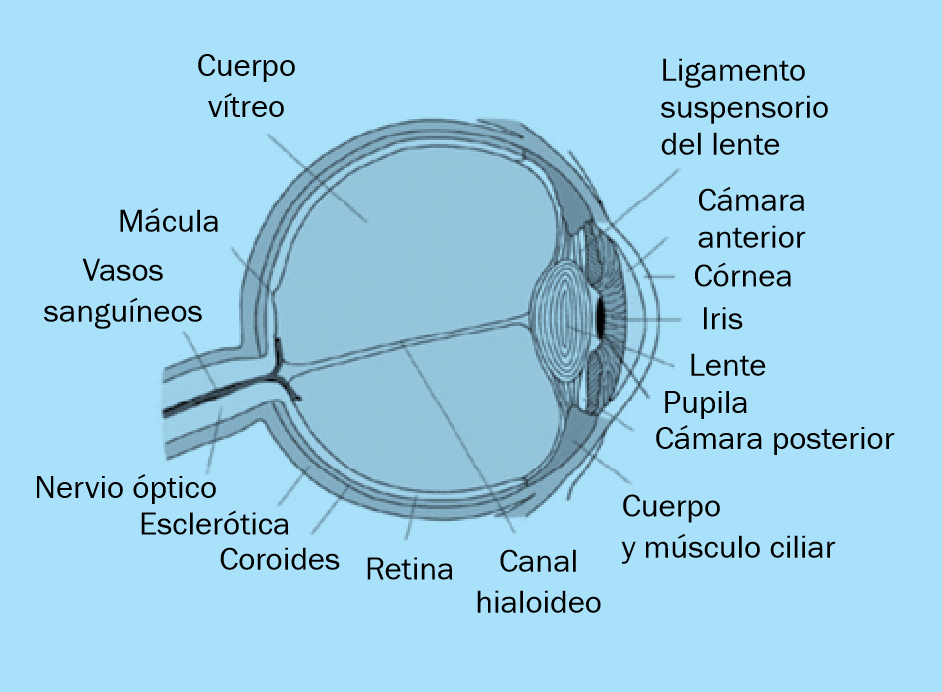
\includegraphics[width=0.45\textwidth]{imaxes/ojo1.png}
    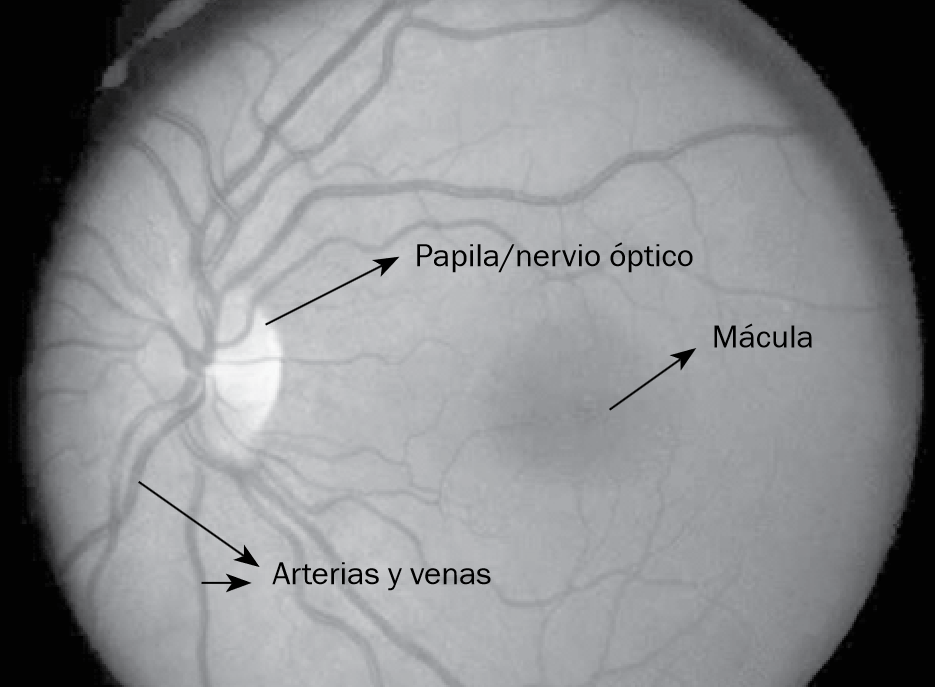
\includegraphics[width=0.45\textwidth]{imaxes/ojo2.png}
    \caption{Imaxes do ollo humano, extraídas de \cite{visionyojo}. Á esquerda, vista lateral do ollo anotada. Á dereita, retinografía do ollo anotada.}
    \label{fig:imaxes_ojo}
\end{figure}

\subsection{Imaxe oftalmolóxica}
\label{subsec:Imaxe oftalmolóxica}
Existen diversas modalidades de imaxe médica que permiten observar o ollo, cada unha con diferentes propiedades e aplicacións. 
Entre elas inclúense a fotografía de fondo de ollo, a tomografía de coherencia óptica (OCT) e a angiografía con fluoresceína \cite{ilginis2014ophthalmic}.

Este traballo céntrase na fotografía de fondo de ollo entre outras razóns polo seu uso común na práctica clínica.
Isto é débese en gran parte á súa accesibilidade, requerindo equipo maís barato e menor entrenamento comparada cas outras modalidades. 
Ademais, é unha técnica non invasiva e rápida de realizar, o que a fai preferible na maioría dos casos \cite{retinimaging}.

Para realizala faise uso dunha cámara especial denominada retinógrafo, e xeralmente require da previa dilatación da pupila do paciente.
Desta forma permítese maior entrada de luz nos ollos, o que provoca unha mellor visualización da retina e mellora a calidade da imaxe.
Un especialista pode analizar a retinografía para detectar signos de enfermidades como a retinopatía diabética, a hipertensión ou a dexeneración macular \cite{retreggood}.

\section{Rexistro de imaxes}
\label{sec:Rexistro de imaxes}
O rexistro de imaxes é un proceso que consiste en, sobre dúas ou mais imaxes, determinar a correspondencia espacial entre elas
 e alinealas nun sistema de coordenadas común, co obxetivo de que as características de interese se atopen na mesma posición.

 Por exemplo, no caso do stitching de fotografías panorámicas, o rexistro de imaxes permite identificar correspondencias entre puntos característicos en múltiples tomas solapadas
  e axustar a súa posición relativa nun marco común. Esta etapa é necesaria para a posterior fusión das imaxes, de modo que as distintas vistas se aliñen con precisión, producindo un resultado final continuo e sen irregularidades visuais.

O rexistro de imaxes ten utilidade en moitos campos diferentes como a imaxe satelital, xeografía, robótica... \cite{goshtasby2017theory} mais o 
campo da imaxe médica é dos mais interesantes póla súa aplicación práctica e é o que se aborda neste traballo.

No ámbito da saúde un rexistro adecuado pode empregarse para comparar imaxes dun mesmo paciente tomadas en distintos momentos, en distintas modalidades ou para comparar entre diferentes pacientes.
Isto permite a revisión do avance dunha enfermidade ao longo do tempo, a fusión de imaxes de distintas modalidades ou a detección de patróns comúns entre distintos individuos.
A fusión de imaxes permite interpretar moito mellor a información dispoñible nelas, e é de gran axuda para guiar aos médicos na toma de decisións.
Tamén é útil para correxir os movementos involuntarios do paciente durante a adquisición de imaxes, como no caso da respiración en imaxes de pulmóns.
As imaxes poden variar a nivel temporal, espacial, de dimensión ou de modalidade.

Tamén é fundamental para a intervención guiada por imaxe (telecirurxía, (\gls{IGRT})) que non 
podería funcionar sen a utilización axeitada de técnicas de rexistro de imaxes. \cite{wang2022neuralrenderingstereo3d}

Ata recentemente, gran parte do traballo de rexistro facíase de forma manual por expertos con software como BigWarp \cite{bigwarp}, 
e dependía das habilidades do profesional para detectar as características de interese e realizar o aliñamento.
Isto facía que o proceso fose lento e propenso a erros, ademais de pouco práctico para grandes volumes de imaxes.

O rexistro de imaxes pode ser clasificado en distintas categorías segundo as súas características:
\cite{deeplernreview3dreg}, \cite{bharati2022deeplearningmedicalimage}
\ref{fig:categorias_de_rexistro}



\begin{figure}[hp!]
    \centering
    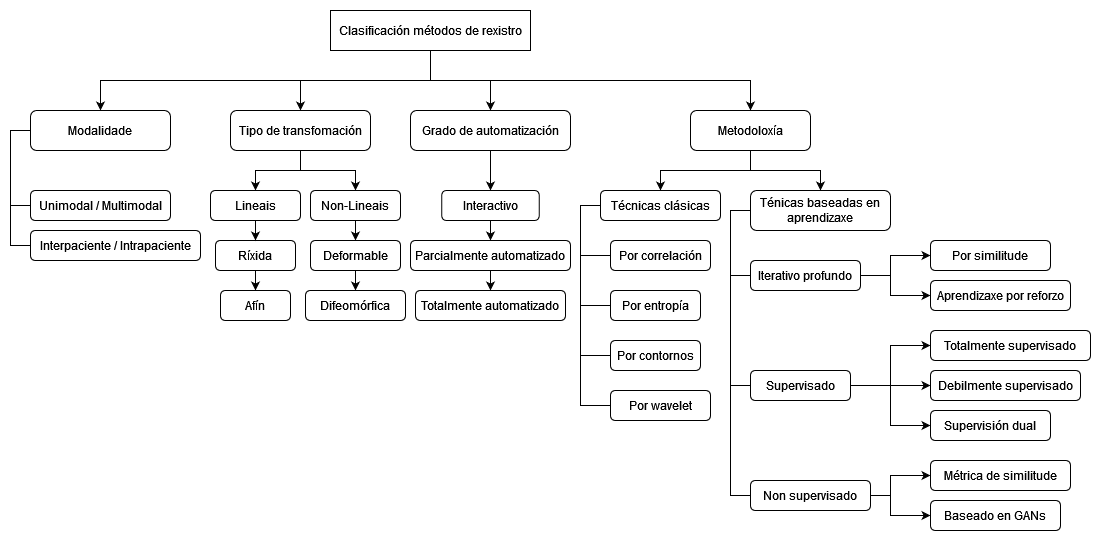
\includegraphics[width=1\textwidth]{imaxes/catreg.drawio.png}
    \caption{Categorías de rexistro}
    \label{fig:categorias_de_rexistro}
\end{figure}

No caso de traballar con dúas imaxes, a imaxe de referencia denomínase imaxe fixa (f) e a imaxe que se quere rexistrar imaxe móbil (m).
Dependendo do tipo de transformación utilizada esta pode ser clasificada en ríxida, afín ou deformable.
A ríxida tan só permite rotación e traslación, mentres que a afín permite ademais escalado e cizallamento.
Ámbas transformacións poden ser representadas por unha matriz de 2 dimensións xa que son deformacións lineais.
Ao contrario, a transformación deformable é non lineal, polo que require dunha dimensión adicional ás da imaxe a rexistrar (unha imaxe de 2d require unha matriz 3d).

Esta matriz denomínase campo de vectores de deformación (DFV), e permite representar deformacións locais na imaxe, facendoa moito mais flexible para representar transformacións complexas e detalladas.
\dots más de DFV \dots

Dentro da deformables poden distinguirse entre transformacións difeomórficas e non difeomórficas.
As transformacións difeomórficas son aquelas que son continuas, invertibles e diferenciables en todo o seu dominio.
Se non tén esta característica, non se pode garantir que a información da imaxe móbil se manteña intacta tras a transformación.
Por iso as transformacións difeomórficas son preferidas en moitos casos \cite{han2022diffeomorphicimageregistrationneural}, 

Existen diversos métodos para realizar aliñamento de imaxes, que poden estar automatizados en maior ou menor medida, sendo moitos deles híbridos. \cite{deeplernreview3dreg}


\subsection{Estado da arte}
\label{subsec:Estado da arte}

Pese á gran cantidade de avances que está a ocorren no campo do aprendizaxe profunda, os métodos clásicos de rexistro de imaxes seguen a ser o estado da arte na maioría de casos, 
principalmente debido á importancia da precisión e a robustez en imaxe médica.


\subsubsection{Métodos clásicos}
\label{subsubsec:Métodos clásicos}

Pese á gran cantidade de avances que está a ocorren no campo do aprendizaxe profunda, os métodos clásicos de rexistro de imaxes seguen a ser o estado da arte na maioría de casos, 
principalmente debido á importancia da precisión e a robustez en imaxe médica. \cite{}

Tradicionalmente impregáronse métodos iterativos baseádos na extracción de características 
seguido dun proceso de optimización entre cada par de imaxes. 
Isto require recoñecer as características de interese en cada imaxe e utilizar unha métrica de similitude 
para determinar a calidade do rexistro.
O proceso consiste en calcular o grado de semellanza entre as imaxes e 
actualizar os parámetros da transformación de forma iterativa utilizando algún mecanismo de optimización
 ata que se cumpran os criterios de terminación.
O resultado final pode ser os parámetros da transformación ou a imaxe fusionada.
A figura \ref{fig:rexistro_iterativo} mostra un diagrama do proceso de rexistro iterativo.

A principal desventaxa destes métodos é a súa lentitude, xa que requiren varias iteracións para converxer.
Non obstante, son moi precisos e robustos, polo que aínda se empregan en moitos casos.

\begin{figure}[hp!]
    \centering
    \begin{tikzpicture}[node distance=2cm, scale=0.8, every node/.style={transform shape}]
        % Nodes
        \node (imageFixa) [process] {Imaxe Fixa};
        \node (imageMobil) [process, right of=imageFixa, xshift=3cm] {Imaxe Móbil};
        \node (featureExtraction) [process, below of=imageFixa, yshift=-1cm] {Cálculo de medida de similitude};
        \node (parameterUpdate) [process, below of=featureExtraction, yshift=-1cm] {Actualización de Parámetros};
        \node (applyTransformation) [process, below of=parameterUpdate, yshift=-1cm] {Aplicar a Transformación};
        \node (criteriaCheck) [decision, below of=applyTransformation, yshift=-1cm] {Criterios Cumplidos?};
        \node (result) [process, below of=criteriaCheck, yshift=-1cm] {Resultado};
        % Arrows
        \draw [arrow] (imageFixa) -- (featureExtraction);
        \draw [arrow] (imageMobil) -- (featureExtraction);
        \draw [arrow] (featureExtraction) -- (parameterUpdate);
        \draw [arrow] (parameterUpdate) -- (applyTransformation);
        \draw [arrow] (applyTransformation) -- (criteriaCheck);
        \draw [arrow] (criteriaCheck) -- node[anchor=west] {Sí} (result);
        \draw [arrow] (criteriaCheck.east) -- ++(1,0) node[anchor=south, xshift=0.5cm] {No} |- (featureExtraction.east);
    \end{tikzpicture}
\caption{Proceso de rexistro de imaxes iterativo}
\label{fig:rexistro_iterativo}
\end{figure}

No proceso de extracción de características destacan algoritmos de SIFT \cite{sift}, SURF \cite{surf}, BRISK \cite{brisk} ou FREAK \cite{freakkeypoint}.

Para encontrar a correspondencia entre os puntos característicos das imaxes, empreganse algoritmos como RANSAC \cite{ransac} ou FLANN \cite{flann}.

Tamén existen múltiples programas que facilitan o rexistro de imaxes, como \cite{simpleitk}, Elastix \cite{elastix} ou ANTs \cite{ants}.


\subsubsection{Métodos de aprendizaxe profunda}
\label{subsubsec:Métodos de aprendizaxe profunda}

Ca chegada dos métodos de aprendizaxe profunda á imaxe médica, comezaron a empregarse redes neuronais para realizar o aliñamento de imaxes.
Estos métodos tenden a ser mais rápidos que os métodos convencionais, a custo de algo de precisión. 
Ademais, estos métodos requiren dunha gran cantidade de datos para ser adestrados, 
o que pode ser unha desventaxa xa que en moitos casos non se dispoñen de bases de datos anotadas do tamaño necesario.

Unha aproximación común é empregar estes conxuntos de datos para optimizar unha CNN que,
 dadas dúas imaxes novas e non vistas, predice o DFV correspondente.

Durante o proceso de entrenamento, a rede ten acceso aos DFVs ca deformación correcta,
 ou pódense obter indirectamente a través da optimización dunha métrica de similitude de imaxes [].

Existen moitas extensións a esta aproximación, como o uso de múltiples etapas ou o uso de redes adversarias durante o entrenamento.

Tamén se propuxeron métodos híbridos que combinan a optimización iterativa ca aprendizaxe profunda, 
entrenando unha CNN nova por cada parella de imaxes. Desta forma conséguese evitar a necesidade de grandes conxuntos de datos para o adestramento.

Os métodos de aprendizaxe profunda poden ser clasificados en dous tipos según se requiran de DFVs anotados ou non na etapa de entrenamento: 
supervisados (requíren de DFVs anotados) e non supervisados (non requíren de DFVs anotados).

Existe un gran interés polos métodos baseados en aprendizaxe profundo, como se reflexa no crecente número de publicacións no campo \ref{fig:method_comp}.

\begin{figure}[hp!]
    \centering
    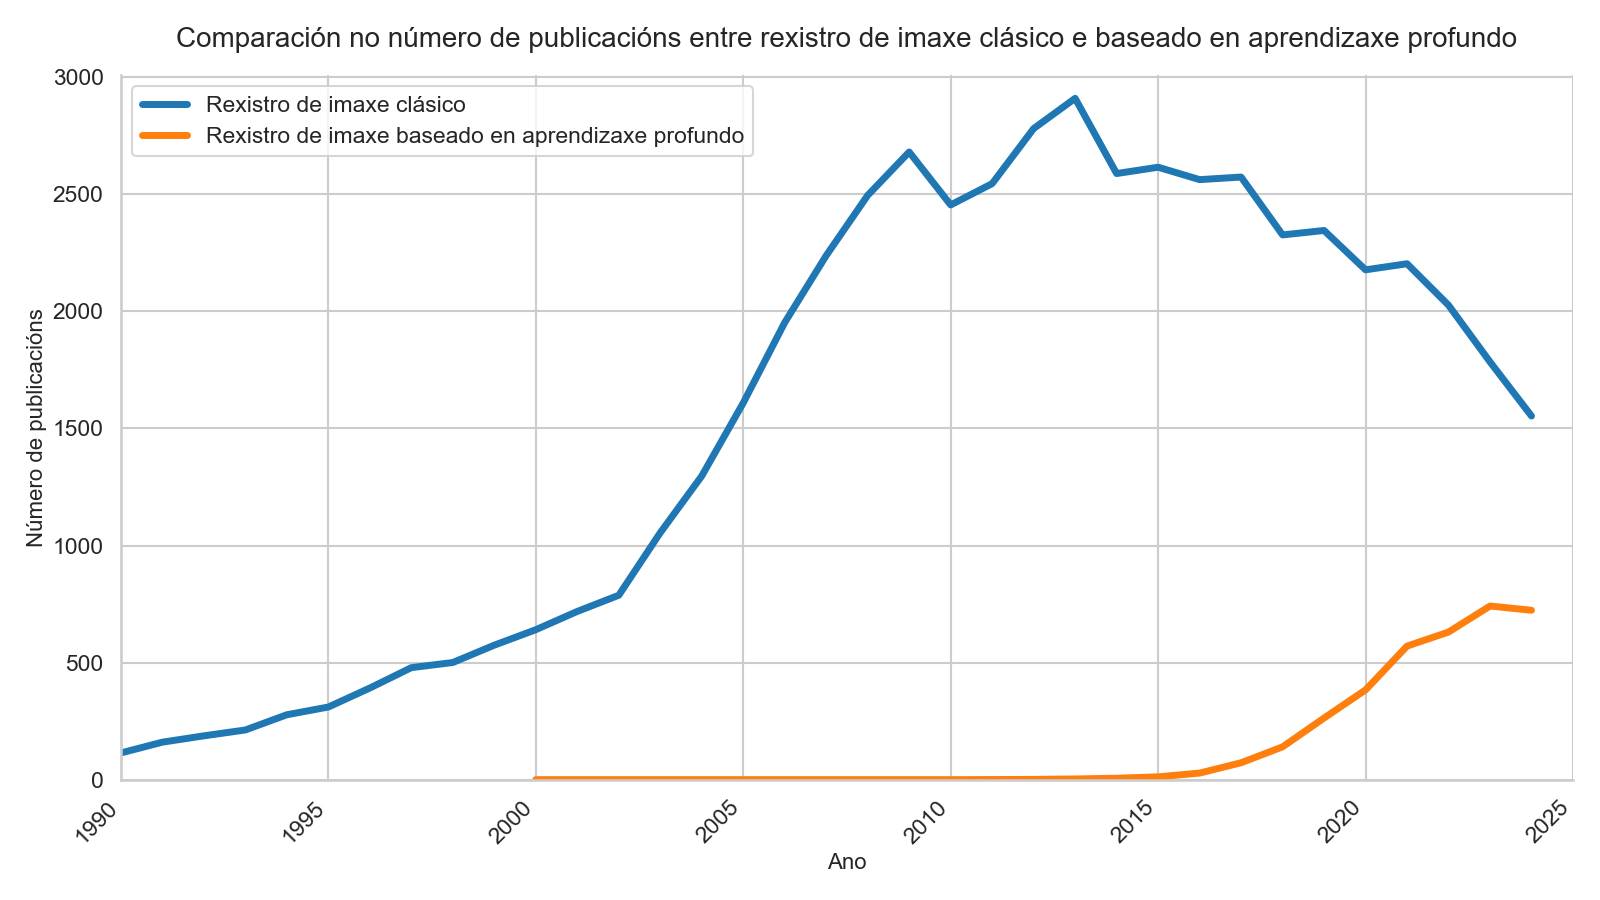
\includegraphics[width=0.8\textwidth]{imaxes/methods_comp.png}
    \caption{Comparación de pubicacións ó longo do tempo que relacionadas co rexistro de imaxes. Datos extraídos de \cite{scopus}, realizando as consultas: "TITLE-ABS-KEY(image AND registration) AND NOT(deep AND learning)" e "TITLE-ABS-KEY(image AND registration) AND (deep AND learning)"}
    \label{fig:method_comp}
\end{figure}

\subparagraph{Métodos Supervisados}
\label{subparagraph:Métodos Supervisados}

Existen dúas subcategorías según o grado de supervisión utilizado na etapa de entrenamento: totalmente supervisados ou débilmente supervisados.
O rexistro totalmente supervisado fai uso de DVFs de referencia para supervisar o proceso de aprendizaxe.
 O termo de perda adoita basearse na discrepancia entre os DVFs de referencia e os DVFs predicidos.
 
No lugar dos DVFs de referencia, o rexistro débilmente supervisado pode utilizar outras etiquetas de referencia implícitas.
 Estas etiquetas non se basan en datos explícitos como os DFVs, senón que utilizan información indirecta para guiar o proceso de rexistro, como a semellanza entre as imaxes ou restricións baseadas na forma ou límites anatómicos das estruturas.
 Máis de dous tipos de datos de referencia son frecuentemente utilizados para adestrar modelos de rexistro débilmente supervisados. \cite{bharati2022deeplearningmedicalimage}
\dots

\subparagraph{Métodos Non Supervisados}
\label{subparagraph:Métodos Non Supervisados}

Un dos maiores retos para entrenar redes efectivas con imaxes médicas é a recolección de datos anotados de calidade para o adestramento \cite{medicalimageanalysis}.
A creación de conxuntos de DFVs anotados é un proceso laborioso e costoso, que normalmente sólo póde ser executado por especialistas, polo que os métodos de rexistro non supervisados son de gran interese.
Xa que a imaxen fixa e a imaxe móbil xa conteñen toda a información necesaria para un rexistro correcto, os métodos non supervisados parecen mais adecuados para a tarefa de rexistro.
De forma similar aos métodos iterativos, é común empregar unha métrica de similitude entre as imaxes xunto con un termo de regularización para guiar o proceso de optimización evitando caer en transformación non realistas.

\cite{Balakrishnan_2019voxelmorph} é un dos métodos mais recoñecidos de rexistro de imaxes non supervisado facendo uso de CNNs.

O rexistro non supervisado de imaxes médicas utilizando GANs é unha subcategoría desta técnica.

\subsection{En retinas}
\label{subsec:Retinas}

Os métodos que funcionan ben en moitos dominios de imaxe médica (cerebro, pulmóns, etc) 
adoitan requirir de axustes para funcionar en retinas, polo que en imaxe oftalmolóxica hai un estado do arte paralelo.
O rexistro mediante landmarks segue a ser moi usado neste contexto, e Hay especial interese por métodos moi robustos que permitan
 o rexistro e fusión de imaxes de diferentes modalidades, por exemplo entre imaxes de fondo do ollo e anxiografías.

\gls{GDB-ICP} é un dos métodos tradicionalmente mais utilizados, proposto por \cite{GDB-ICP}, consiste en
 comezar cunha ou máis estimacións iniciais que só son precisas en pequenas rexións da imaxe, chamadas rexións bootstrap. 
 En cada rexión bootstrap, o algoritmo itera sobre os seguintes pasos: 
 
1: refina a estimación da transformación usando restricións só dentro da rexión bootstrap; 
2: expande a rexión bootstrap;
3: comproba se se pode usar un modelo de transformación de orde superior, deténdose cando a rexión se expande para cubrir a superposición entre imaxes.


\cite{piifd} propón un framework nomeado Harris-PIIFD no cal comezan por detectar os puntos de esquina como candidatos a puntos de control utlizando Harris \cite{Harris1988ACC}.
Posteriormente, introdúcen o algoritmo \gls{PIIFD} para describir os puntos característicos, e aplícase o algoritmo \gls{BBF} \cite{BBF} para identificar coincidencias entre pares de imaxes.
Finalmente, refínanse as coincidencias e elimínanse as incorrectas, e escóllese o tipo de transformación a aplicar en función do número de coincidencias.
A transformación máis sinxela (ríxida) require polo menos dous pares de puntos de control. Se o número de coincidencias é maior ou igual a tres pero menor que seis, aplícase a transformación afín; e se o número é maior ou igual a seis, aplícase a transformación polinomial de segunda orde.

Varias melloras a este método foron propostas, como \cite{ur-sift}, que introduce o algoritmo \gls{UR-SIFT-PIIFD}, que combina UR-SIFT con Harris-PIIFD para extraer puntos invariantes á escala e obter unha maior robustez.
\cite{GMM} propón un método baseado en \gls{GMM} para a extracción de puntos de control, que demostra ser mais robusto que os métodos anteriores, especialmente en imaxes con mala calidade ou pouca solapación.
\cite{MFSP} constrúen sobre os modelos anteriores e utilizan \gls{SURF} para a extracción de puntos de control e \gls{PIIFD} para a descrición dos mesmos, 
logo presentan \gls{MFSP}, un método non ríxido que combina a preservación de estrutura cos puntos característicos para o rexistro das imaxes. 
A transformación final efectúase mediante \gls{TPS} \cite{TPS}.

\gls{REMPE} \cite{rempe} propón a estimación simultánea da pose das cámaras que adquiriron as imaxes e da forma e pose do ollo. Utiliza un modelo elipsoidal para u ollo e estima a posición das cámaras inicialmente mediante RANSAC, seguido de una variante de \gls{PSO} \cite{pso} para refinala. 
Versións anteriores deste método utilzaron modelos esféricos en lugar de elipsoidais, e \gls{SURF} en lugar de SIFT \cite{H-M16}.


\ref{fig:retin_reg}
\begin{figure}[hp!]
    \centering
    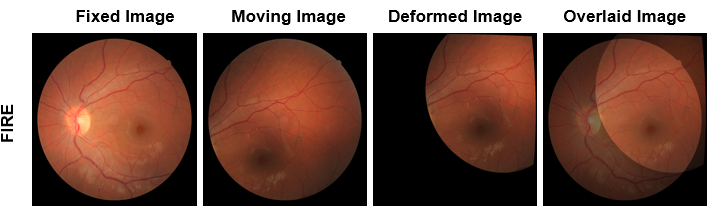
\includegraphics[width=0.8\textwidth]{imaxes/retin-reg.png}
    \caption{Exemplo de rexistro de imaxes de retina \cite{sivaraman2024retinaregnetzeroshotapproachretinal}}
    \label{fig:retin_reg}
\end{figure}


\section{Representación Neuronais Implícitas}
\label{sec:Representación Neuronais Implícitas}
 
A representación de coñecemento é un dos problemas máis importantes na área da computación, e as 
redes profundas son unha das ferramentas máis útiles, especialmente no campo da visión por computador.
Tradicionalmente empréganse representacións discretas, onde o espazo de entrada é dividido en celdas e cada celda é asignada un valor (por exemplo nubes de puntos, matrices de píxeles ou vóxeles...).
Unha das principais desventaxas destas representacións é que a súa complexidade increméntase rápidamente co número de dimensións representadas, ademais do custo de memoria asociado.

 As representacións neuronais implícitas son un paradigma innovador que permite modelar sinais continuas mediante funcións parametrizadas por redes neuronales.
 Codifican a información como unha función continua, que mapea valores de entrada aos valores correspondientes de saída, en lugar de almacenar directamente valores de características o señales.

Representar o sinal como una función continua permite solucionar os problemas asociados á discretización e obtéñense outra serie de vantaxes.

As INR son moito mais eficientes debido á compresión da información que realizan de forma implícita. Ao mesmo tempo, permite un nivel de detalle non limitado pola resolución da imaxe, senón pola capacidade da rede. 
 Ademais, as representacións continuas son diferenciables, o que permite o cálculo de gradientes e derivadas de forma analítica en lugar de ter que aproximalos por diferencias finitas.
 Isto tamén implica que as representacións implícitas son independentes da resolución, o que permite a reconstrucción en calquer escala espacial.
 
Tipicamente emprégase un MLP como architectura para representar a función implícita. Non obstante, o uso da función de activación ReLU tende a non obter os mellores resultados \cite{rahaman2019spectralbiasneuralnetworks},
polo que moita investigación diríxese a atopar alternativas que melloren a representación do sinal. \cite{essakine2024standimplicitneuralrepresentations}

Por exemplo SIREN \cite{sitzmann2020implicitneuralrepresentationsperiodic}, sobre a que profundizaremos mais adiante.
\cite{ramasinghe2022periodicityunifyingframeworkactivations} propón as funcións de activación gaussianas como alternativa a SIREN, e argumenta que poden obter mellores representacións e mais robustas.
\cite{saragadam2023wirewaveletimplicitneural} achega unha nova función de activación baseada en wavelets, que demostra ser especialmente útil para a representación de imaxes.

As representacións implícitas poden ser clasificadas en dúas categorías: generalizables e sobreajustadas \cite{yu2024neuraltrajectorymodelimplicit}. 
As representacións sobreaxustadas céntranse en reproducir con precisión unha única sinal, mentres que as representacións generalizables poden modelar varias.

As INR son utilizadas en todo tipo de campos, dende xeración de imaxes \cite{reddy2022multiimplicitneuralrepresentationfonts}, pasando por
reconstrucción de obxetos \cite{mildenhall2020nerfrepresentingscenesneural} \cite{mescheder2019occupancynetworkslearning3d} ou modelado de sinais complexas \cite{wu2021iremhighresolutionmagneticresonance}.

As representacións implícitas están a recibir cada vez máis atención da comunidade médica \cite{molaei2023implicitneuralrepresentationmedical}, e son 
especialmente útiles para as tarefas de imaxe inversa, que requiren a reconstrucción de representacións correctas a partir de datos incompletos ou ruidosos. 
No caso de \cite{shen2023nerpimplicitneuralrepresentation}, propuxeron unha representación implícita para a reconstrucción de imaxes de resonancia magnética a partir de datos incompletos facendo uso de redes implícitas, 
e obtiveron resultados comparables a métodos tradicionais.

\cite{mildenhall2020nerfrepresentingscenesneural} propuxeron unha representación implícita para a representación de escenas 3D, 
 optimizando unha función volumétrica continua que modela a densidade de volume e a radiancia emitida en cada punto do espazo.
 Utilizando un MLP, cuxa entrada é unha única coordenada continua 5D (localización espacial (x, y, z) e dirección de visión (θ, φ)) 
 e cuxa saída é a densidade de volume e a radiancia emitida dependente da vista nesa localización espacial. 
A única entrada necesaria para optimizar a súa representación é un conxunto de imaxes con poses de cámara coñecidas. 
Demostrando que as representacións implícitas están capacitadas para modelar escenas 3D complexas con alta fidelidade visual.
 
As representacións implícitas teñen bastante potencial no campo de planificación de traxectorias, como demostran \cite{yu2024neuraltrajectorymodelimplicit} e \cite{trajectinr}, 
que propóñen o uso de INRs para modelar entornos e planificar traxectorias para un ou varios axentes.
A principal vantaxe de facelo desta forma frente á forma tradicional (algoritmos computacionalmente intensos, especialmente para multi-axentes) é a velocidade á que encontran solucións (por debaixo do milisegundo en GPUs).
A maior desventaxe é que non garanten a converxencia a unha solución óptima e sen colisións, mais os autores demostran que a calidade das traxectorias xeradas é comparable ás obtidas é adecuada para a maioría das aplicacións.

Mais especificamente, en \cite{teleoperatdrob} utilizan este tipo de representacións para garantir a seguridade do paciente durante a cirurxía teleoperada e optimizar a traxectoria do robot para evitar colisións co paciente, neste caso na boca e gorxa.
Con este método, evítase a reconstrución de mallas a partir de imaxes, que é un proceso costoso e imperfecto, e modélase mediante unha INR a partir dos datos médicos dispoñibles.
Os comandos de movemento da man do operador son tomados como entrada polo modelo, que logo de un proceso de optimización, xera unha secuencia de movementos libre de colisións que será enviada á man robótica.

Coin [18] compress an image by storing the
weights of a neural field overfitted to it.

\cite{velikova2024implicitneuralrepresentationsbreathingcompensated} and  casos de uso interesantes.

Tamén se empregan en segmentación, compresión e síntesis de imaxes.

 No caso do aliñamento de imaxes, buscase optimizar a función que mapea cada localización da imaxe fixa a unha localización da móbil.
 

\section{IDIR}
\label{sec:IDIR}
IDIR (Implicit Deformable Image Registration) é un método de aliñamento de imaxes baseado en redes neuronais. 
A súa principal diferenza frente a unha rede convolucional tradicional é que, 
en lugar de predicir a transformación entre imaxes, optimízase unha rede para esta mesma represente esta transformación.

O que \cite{wolterink2021implicit} propón é optimizar directamente o DFV facendo uso
 dunha representación implícita, de forma que a deformación está representada nos propios pesos dunha MLP.

 \cite{sun2024medicalimageregistrationneural} e \cite{nodeo} propuxeron métodos de rexistro de imaxes similares de forma independente,
 baseados en Neural ODE (ODE-Nets)\cite{neuralode}, unha familia de modelos de aprendizaxe profundo que trata a rede como un sistema continuo en lugar de unha secuencia de capas discretas.


\subsubsection{Arquitectura}
\label{subsubsec:Arquitectura}

Faise uso dun MLP de 3 capas, e determinaron experimentalmente que obtiñan mellor resultado con 256 unidades por capa que 128.
Por cada epoch de entrenamento (2500 en total), 10000 puntos son muestreados aleatoriamente do espazo de coordenadas dentro da máscara.
O término de perda é a 'normalized cross-correlation' entre os valores dos píxeles muestreados na imaxe fixa e os correspondentes da imaxe móbil.
Utilizan Adam de optimizador, cun learning rate de 0.0001.

\subsubsection{Función de activación}
\label{subsubsec:Función de activación}

Unha elección estándar para a función de activación é ReLU: σ(x) = max(0, x). 
Non obstante, para redes de representación implícita como ca que estamos traballando, esta ten unha serie de desventaxas.

Sen embargo, as ReLUs teñen un sesgo cara a sinais de baixa frecuencia \cite{rahaman2019spectralbiasneuralnetworks}, 
 o que significa que o modelo pode ter dificultades para representar pequenas deformacións locais no rexistro de imaxes.
 
Existen varias formas de superar este sesgo, como preprocesar as coordenadas de entrada con funcións de activación periódicas \cite{mildenhall2020nerfrepresentingscenesneural} 
ou substituír a función de activación ReLU por unha función de activación periódica \cite{sitzmann2020implicitneuralrepresentationsperiodic}.
Neste traballo escollemos a segunda opción, utilizando unha función de activación periódica para obter un modelo de tipo SIREN, σ(x) = sin(x).
Unha vantaxe engadida das funcións de activación periódicas nas redes SIREN é que poden ser diferenciadas varias veces, 
o que expande substancialmente o conxunto de termos de regularización que se poden empregar na rede, como veremos na seguinte sección.

\cite{mildenhall2020nerfrepresentingscenesneural} non utiliza unha función de activación periódica, mais para a representación adecuada de zonas de alta frecuencia 
utilizaron positional encoding, que xa as incorpora de forma implícita na rede con bós resultados. \ref{chap:Positional Encoding}

\subsubsection{Termos de regularización}
\label{subsubsec:Termos de regularización}

Debido a que el registro de imágenes deformables es un problema mal planteado (ill-posed problem**), 
es común regularizar el DVF para evitar deformaciones poco realistas.
 Los métodos de registro basados en redes neuronales convolucionales (CNN) representan los DVF 
 como muestras en una cuadrícula de vóxeles, y por lo tanto, solo pueden aproximar gradientes espaciales
 mediante esquemas de diferencias finitas. Esto conlleva errores de discretización y pérdidas de precisión.

Facendo uso de representacións implícitas, todas as operación son diferenciables, e os gradientes poden
 ser computados de forma analítica en lugar de ter que aproximalos.
Utilizando ReLU como función de activación, a rede é diferenciable unha vez, mentres que utilizando
 unha función de activación periódica (como SIREN), a rede é diferenciable varias veces.
Desta forma, podemos calcular calquera número de termos de regularización e incluilos na optimización da rede.

Algúns exemplos de termos de regularización que se poden empregar son:
\begin{itemize}
    \item Jacobian regularizer: 
    O determinante Jacobiano da transformación (det ∇Φ) nunha localización x é un indicador de estiramento ou compresión local.
    Un determinante Jacobiano negativo indica que está a ocurrir folding e a transformación non será invertible.
    \dots

    \item Hyperelastic regularizer
    Tamén se póden engadir restricións ao DVF con este termo proposto por \cite{HyperelasticRegularization}.
    Consiste en tres termos, un termo de lonxitude, un termo de área e un termo de volumen co obxetivo de controlar variacións nestes aspectos.
    O termo de lonxitude penaliza a variación da lonxitude dos vectores do DVF e está controlado pola matriz do Jacobiano da transformación.
    A matriz de cofactores e o determinante da matriz do Jacobiano da transformación controlan a área e o volume respectivamente, 
    penalizando o crecemento e a contracción por igual.
    \dots

    \item Bending energy penalty
    Pódese impoñer a suavidade do DVF empregando esta penalización proposta en (Rueckert et al., 1999).
    Require que as segundas derivadas do DVF sexan pequenas en todo o dominio, 
    polo que non pode ser utilizado nunha rede que utilice ReLU como función de activación (a segunda derivada de unha ReLU é sempre igual a 0).
    \dots
\end{itemize}


\subsubsection{Método}
\label{subsubsec:Método}

Sendo o obxetivo encontrar unha transformación espacial óptima entre a imaxe fixa e a imaxe móbil,
é necesario obter a función de deformación  Φ(x) = u(x) + x que mapea cada coordenada x na imaxe fixa a unha coordenada na imaxe móbil, 
de forma que a coordenada x na imaxe fixa corresponda anatomicamente á coordenada Φ(x) na imaxe móbil.
Este problema pode ser formulado como un problema de optimización onde Ldata é unha métrica de similitude entre as imaxes fixa e móbil, Lreg é un termo de regularización na transformación Φ, e α é un termo de ponderación.
\begin{equation}
   \hat{\Phi} = \operatorname*{Arg\,min}_{\Phi} L_{data}(M \circ \Phi, F) + \alpha L_{reg}(\Phi)
\end{equation}

A aportación clave é que a transformación Φ está implícitamente representada nunha rede neuronal.

Comparado cunha CNN tradicional, esta rede non recibe valores de intensidade de píxel como entrada,
senón que recibe coordenadas espaciais (continuas) e devolve unha nova coordenada.
Xa que os pesos da rede definen a transformación, estos poden ser optimizados directamente 
facendo uso dunha métrica de similitude como función de perda.

Parametrizar a función de deformación como unha INR dentro dun MLP ten varias vantaxes para o rexistro de imaxes.
En primeiro lugar, a representación da transformación é continua e polo tanto independente da resolución da imaxe, 
grazas a iso o mesmo modelo poder ser empregado para imaxes de calquer tamaño, ao contrario dunha CNN tradicional 
que ten que ser adaptada para cada resolución.

Segundo, facelo desta forma permite aproveitar as capacidades de librerías como PyTorch para calcular os gradientes da transformación respecto das coordenadas.
Isto permite obter gradientes máis precisos que as aproximacións por diferencias finitas 
e permite aproveitar unha gran cantidade de literatura sobre regularización eficientes en imaxes médicas.

Terceiro, pódese modificar a función de activación empregada na rede para axustala ás necesidades particulares da tarefa de rexistro de imaxes.
Neural Tangent Kernel (NTK) es un concepto que describe cómo un modelo de red neuronal responde a cambios en sus parámetros durante el entrenamiento,
e dependendo da función de activación empregada, o NTK varía e a rede pode ser máis ou menos sensible a certas deformacións.

Finalmente, entrenaráse unha nova rede por cada parella de imaxes, sendo esta unha rede bastante pequena en comparación e precindindo así da necesidade de grandes conxuntos de datos para o seu adestramento.



\section{Traballo proposto}
\label{sec:Traballo proposto}

Baseándose no framework introducido por \cite{wolterink2021implicit},
 propónse modificalo para adaptalo a imaxes médicas de retina.
